% options:
% thesis=B bachelor's thesis
% thesis=M master's thesis
% czech thesis in Czech language
% english thesis in English language
% hidelinks remove colour boxes around hyperlinks

\documentclass[thesis=M,english]{FITthesis}[2012/10/20]
\setcounter{secnumdepth}{2}
\setcounter{tocdepth}{1}

% \usepackage[utf8]{inputenc} % LaTeX source encoded as UTF-8
% \usepackage[latin2]{inputenc} % LaTeX source encoded as ISO-8859-2
% \usepackage[cp1250]{inputenc} % LaTeX source encoded as Windows-1250

\usepackage{graphicx} %graphics files inclusion
% \usepackage{subfig} %subfigures
% \usepackage{amsmath} %advanced maths
% \usepackage{amssymb} %additional math symbols
\usepackage{listings}
\usepackage{dirtree} %directory tree visualisation
\usepackage{capt-of}

% % list of acronyms
% \usepackage[acronym,nonumberlist,toc,numberedsection=autolabel]{glossaries}
% \iflanguage{czech}{\renewcommand*{\acronymname}{Seznam pou{\v z}it{\' y}ch zkratek}}{}
% \makeglossaries

% % % % % % % % % % % % % % % % % % % % % % % % % % % % % % 
% EDIT THIS
% % % % % % % % % % % % % % % % % % % % % % % % % % % % % % 

\department{Department of Software Engineering}
\title{Mobile application and API server to store points of interest}
\authorGN{Timur} %author's given name/names
\authorFN{Tatarshaov} %author's surname
\author{Ing. Timur Tatarshaov} %author's name without academic degrees
\authorWithDegrees{Ing. Timur Tatarshaov} %author's name with academic degrees
\supervisor{Ing. Josef Gattermayer}
\acknowledgements{I would like to thank my lovely family especially my parents, who made their best to grow me up and gave me a chance to be here and get hight level university degree in Czech Republic. Without their efforts I wouldn't be able to be who I am and where I am. Also I would like to thank people that were close to me throughout my life, all of them made an impact on my being and made changes to my personality.}
\abstractEN{The aim of the thesis is to develop a mobile application that will store points of interests to a server backend. Single points of interests will be shared among users.}
\abstractCS{C{\' i}lem diplomov{\' e} pr{\' a}ci je vypracovat mobiln{\' i} aplikaci kter{\' a} bude ukl{\' a}dat body na server. Bod se m{\. u}{\v z}e p{\v r}en{\' a}{\v s}et mezi u{\v z}ivateli.}
\placeForDeclarationOfAuthenticity{Prague}
\keywordsCS{Geolokace, navigace, mobilní aplikace, API}
\keywordsEN{Geolocation, navigation, mobile application, API}
\declarationOfAuthenticityOption{1} %select as appropriate, according to the desired license


\begin{document}
%\lstlistoflistings
% \newacronym{CVUT}{{\v C}VUT}{{\v C}esk{\' e} vysok{\' e} u{\v c}en{\' i} technick{\' e} v Praze}
% \newacronym{FIT}{FIT}{Fakulta informa{\v c}n{\' i}ch technologi{\' i}}

\setsecnumdepth{part}


\chapter{Introduction}

\section{Motivation}

Nowadays world is a rapidly changing environment. Distances became shorter mostly because of flights. Information is being transferring faster because of digital copies and growth of the worlds network infrastructure. But presence of human being in a particular place in sake of knowledge exchange, work opportunities or traveling is still can't be underestimated. Consequently more and more people find oneself in completely new locations and cities with different urban architecture, lifestyle and language. 

Navigation in a new foreign locations becomes difficult even for a short time stay. Such simple tasks as finding hotel destination, parked bicycle or cozy camping location visited previously may become a problem in unfamiliar areas where existing navigation solutions could be useless.

It is possible to solve those problems of mobile human with existing technologies including hardware and complementary software. Contemporary mobile devices often equipped with location detection hardware chips and tools that provide possibilities to determine devices location even for a third-party applications.



\section{Goal of the project}

Goal of this project is to develop system that will help users to navigate to earlier visited places. System will consist of the mobile application and server application with exposed API and designed with ability to be scaled.

Mobile application will serve user with geolocation positioning and interactions with the server application API by means of networking compatibilities of the device.

Server application will serve the goal of increasing reliability of the system and provide possibility for extension to other platforms without data loss. To enable devices to communicate with server application  will be implemented API or universal interface for managing server data.


%Goal of this project is to develop software solution that will take advantage of existing hardware and let users save their locations and navigate to them later. Rreliablity of the system sould be supported by remote servers application with exposed API.


\setsecnumdepth{all}

\chapter{Analysis of requirements}

\section{Functional requirements analysis}

\subsection{API requirements}

API is a subject designed to be utilized by wide range of devices and platforms. Those different clients and platforms could have different languages and technologies they working with. Even having clients that take advantage of the same technology stack, this stack usually different from server side technologies., because mobile devices by definition have less computation power and resources than servers. API should be designed to be used for a long-term period, which means future and even not in-market devices should be able to utilize implemented API. 

Among advantages of the API as a concept is independence of realization and exact technology stack. Once described and standardized API supposed to be utilized by clients in the same way as time goes by even thought implementation or separate parts could be changed.

Wide range of clients, extensibility, different technology stacks apply set of requirements for the API implementation. According to mentioned constraints technology chosen for implementation should be something that exists on the market and widely used. 
Subject of responsibility of API is to provide interface for managing points of interest on the server. Managing includes operations of creation, reading, updating and deletion, so called CRUD operations.

API should be designed able to distinct clients from each other. Points of interest of the requesting client should be returned to it. That implies support of authentication \cite{auth} by API technology or ability to implement verification of user identity on top of it as at extension.

Different Points of interest should be seen only by owner. Not authenticated user or not owner of data shouldn't  be able to get it.  Above requirements imply support of verification that a user has rights to access a resource or so called authorization \cite{auth} technology. API must provide means to separate user permissions to the data, so foreigners data will not be accessed.

Points of interest of the user should be not only secure on the level of API resources design but also on transport layer. That means user data must not be able to be retrieved by not the way it designed to be. API should provide level of security by encryption or be able to support extension to implement this measures on top of it.

API should be designed to be utilized by mobile devices. Even contemporary phones have limited computation power and limited resources including memory, energy capacity, networking speed. Mobile devices constraints forces to use less redundant format of data used by API possible, to be transferred over relatively slow mobile networking connections faster. Format shouldn't be complicated for processing implying low computation power of mobile devices. 

Mobile devices could be used in different locations where connectivity could be low or absent. That means network connection of mobile devices not only relatively slow but also not permanent. Once connected client and server must not rely on constant availability of that connection and messaging can’t rely on the same state of connection between client and server. With that said API must be stateless or be able to use stateless principle, once reconnected client and server would be able to recognize each other and recreate previously established state of operations.

Unreliable wireless mobile network connection should be taken into account. API technology should provide or take advantage of error prevention technology to be assure data transferred completely and without errors.

Data related to points of interest is textual, so API technology must be able to transfer textual data or convert data to text format and decode from it.

API should be able to inform client about success or failure of the CRUD operation and be able to provide message of error if any to let client to be assure about status of the operation and state of the server data.

API is a middleware technology, which should be most general possible to be able to be consumed by different clients.

Technology should be free to use to enable to implement cheap solution without possible vendor limitations. Ability to develop addition functions in existing software also important.

API must enable clients to manage data related to their points of interest on the server via Internet.

Overview of interaction with API by means of client device is depicted on following schema.

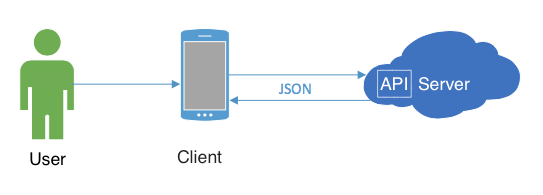
\includegraphics[width=1.0\textwidth]{images/architecture}
\captionof{figure}{Overview of interaction with API}

\subsection{Mobile platform requirements}

Mobile application along with mobile device is a client of API that creates points of interest and interacts with server application by means of implemented API.

Points of interest should include geolocation \cite{geolocation} data that determined by mobile device. It means device should be able to resolve user location in most accurate way possible. To be able to interact with API over network, mobile device should support remote communication and data transferring over the Internet by means of one of the either cellular network, Wi-Fi or other technology. Without that client won't be able to interact with API in a designed client-server manner which requires at least one communication channel.

Mobile device should be able to install third-party software and enable developers of that software take advantages of hardware technologies of mobile device. 

Mobile application must be able to utilize chosen API technology.

\section{Quantitative requirements}

\begin{itemize}
  \item Mobile application must be able to manage up to 1000 points of interest
  \item API must enable client to provide operations on up to 1000 points of interest
  \item Server application must be able to store up to 100000 users
\end{itemize}

\section{Server requirements}

\begin{itemize}
	\item Java 8
	\item MongoDB 3 or higher
	\item Ubuntu 14.10 
	\item Docker 1.6 or higher
\end{itemize}

\section{Mobile requirements}

\begin{itemize}
	\item iPhone 4S or newer or emulator
	\item iOS 8 or higher
	\item Swift 1.2 
\end{itemize}


\section{Comparison of required technologies}


\subsection{Comparison of available API technology solutions}

\subsubsection{SOAP}

SOAP is protocol for messaging of structured information between web services in computer networks.
SOAP can utilize different transfer protocols for communication including but not limited to HTTP, SMTP and FTP. Message in SOAP protocol called envelope.
Data in messages should be text-based or text-encoded.

Technology widely used for encapsulation of objects in Java language. Not broadly supported and used by other languages.

Data is wrapped into XML-based format. That is the only messaging format supported by SOAP which to some extend means redundancy of the transferred envelopes and difficulty to be read by human. XML format is more expensive in terms of computation power for processing compared to number of other formats.
Protocol is stateless or stateful depending on transport protocol.

WSDL is often used in combination with SOAP and an XML Schema to provide web services over the Internet. A client program connecting to a Web service can read the WSDL file to determine what operations are available on the server. That means available API operations could be described in special format, which will enable clients to discover possible API operations and way to access them.


\subsubsection{REST}

REST is a HTTP based technology that was coined by Ted Nelson in 1991 and still widely used. 

RESTful \cite{restapidesign} API supports CRUD operations by design of HTTP protocol it inherits from. Operations is represented by verbs of HTTP. Data could be sent either in request body or query parameters. RESTful API technology is not locked to any messaging format and support different representations of data transferred, limited only by client and server support of it. Such formats could be  JSON, XML and plain text.

REST supports status codes inherited from HTTP. Status codes along with status messages could provide full spectrum of information of client about success or failure of operation and state of the server application.

Data transfered between server and client either textual or encoded to textual. As far as technology is based on HTTP protocol, which is stateless by design, REST inherits this property of it.

HTTP provides by it's extension HTTPS. Security is supported by encryption and packaging transfered data using TLS \cite{tls}. REST could be utilized by HTTPS as well and be secured by it's methods.

Authentication is supported at HTTP level enables to use different mechanisms including following.

\begin{itemize}

	\item HTTP Basic authentication. Username and password pair separated by column base64 encoded. Authentication is being made in one step.
	\item HTTP Digest. No password transfered between a client and a server but a hash value. Authentication is being made in three steps. 
	\begin{enumerate}
		\item Client accesses a protected area
		\item Server requests authentication with 'WWW-Authenticate' header, which contain additional data for the next step, such as quality of protection (QoP)
		\item Client calculates a response hash by using the realm, his/her username, the password, and the QoP and requests the resource with authorization header

	\end{enumerate}

	\item OAuth. Users can grant access to third-party application without exposing their users credentials. Requires existence of authorization server and token endpoints which provide temporal tokens for accessing resources.

\end{itemize}



\subsubsection{Usage statistics}

Following numbers and charts based on usage statistics among protocols could make impact on decision which of them to use for API design.

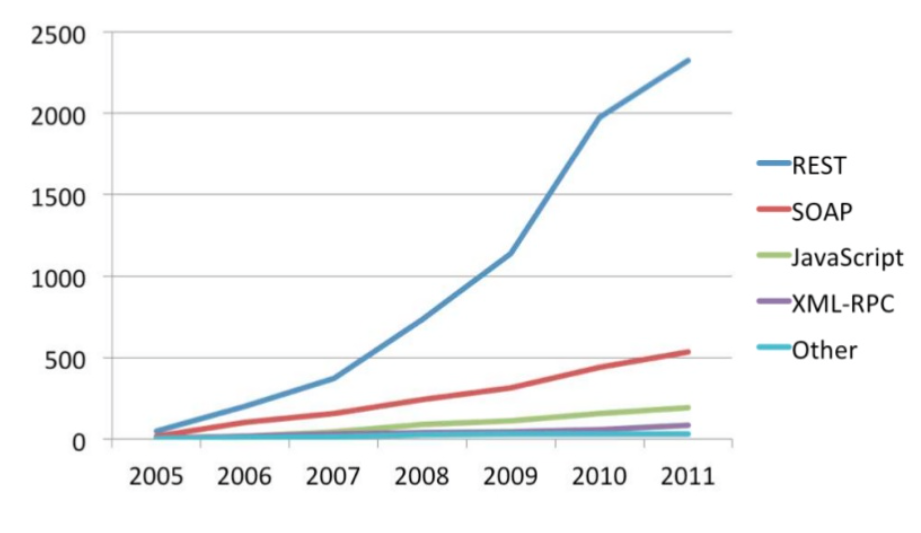
\includegraphics[width=0.9\textwidth]{images/rest_vs_orthers_over_years}
\captionof{figure}{Statistics of usage APIs protocols according to Programmable Web by 2011}

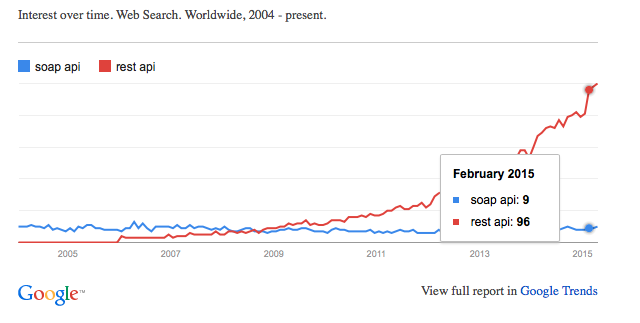
\includegraphics[width=0.9\textwidth]{images/google_trends}
\captionof{figure}{Google search trends: SOAP API and REST API}

Taking into account general API growth and importance of APIs in future web increase of REST API is predictable.

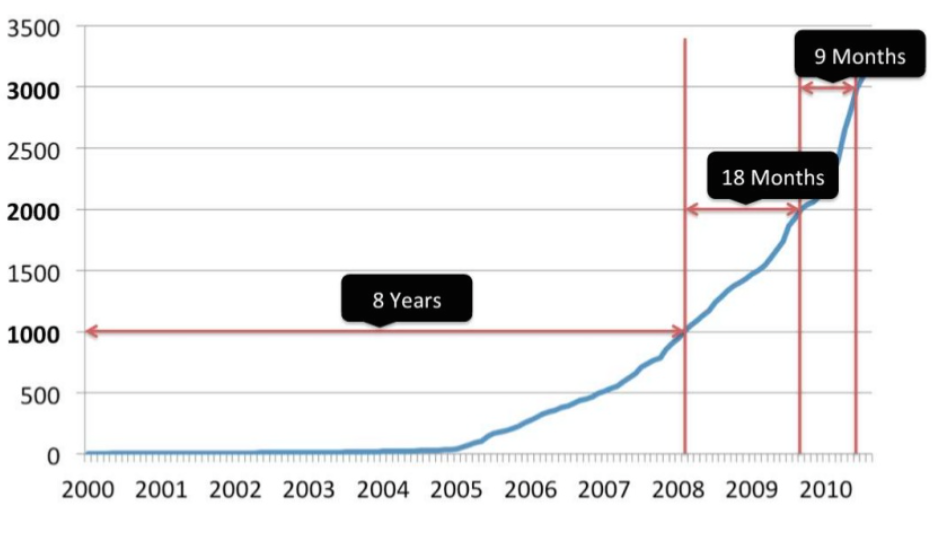
\includegraphics[width=0.9\textwidth]{images/total_apis_growth}
\captionof{figure}{Total growth in number of APIs}

\subsubsection{Choice of API technology}

Several protocols have been reviewed in this chapter. Advantages and disadvantages of them were considered. 
REST for purpose of this project has been chosen. Technology is less verbose than SOAP, let developers use any format for messaging and supported by many languages and clients. REST has been invented decades ago and still widely used due to it's properties to be general and reliable protocol. Technology fulfills requirements of this project completely.

\subsection{Comparison of available transport layer protocols}

\subsubsection{TCP}

TCP is one of the main protocols communication protocols of transport layer of the Internet. It stated to manage data transfer in TCP/IP based networks.

TCP provides mechanism of repeated data request in case of data loss and prevents duplicates of data. Preserve completion of transfered data and informs sender about result.

\subsubsection{UDP}

TCP is one of the main protocols communication protocols of transport layer of the Internet. It enables faster data transfer compared to TCP. Speed up is caused by simplicity of protocol communications. There is no special message for establishing communication channels. Protocol does not ensure completeness and validness of transfered data. Widely used in systems where error prevention is not needed or not important.

\subsubsection{Choice of transport layer protocol}

HTTP usually utilize TCP protocol, which provide error prevention mechanism. Having poor mobile network connectivity TCP could take care of possible network errors. TCP is being used for this project.

\subsection{Comparison of encryption technologies}

\subsubsection{SSL}

SSL is cryptographic protocol designed to provide communications security over a computer network.  It uses asymmetric cryptography to authenticate the counterparty with whom they are communicating, and to negotiate a symmetric key. This session key is then used to encrypt data flowing between the parties.

Currently SSL considered as vulnerable, outdated and suppressed by TLS.

\subsubsection{TLS}

TLS as well as it's predecessor is a public-key based symmetric cryptography for data transfer. In symmetric public-key cryptography each party generates a public/private key pair and distributes the public key. After obtaining an authentic copy of each other's public keys, parties can compute a shared secret offline, which can be used as a key.

\begin{center}
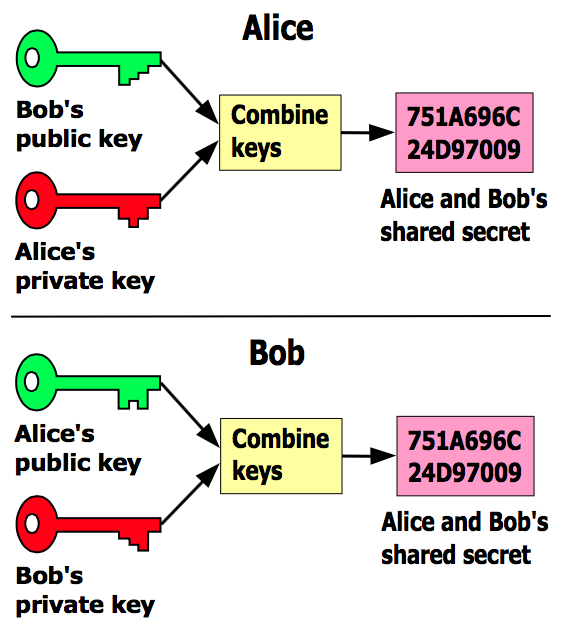
\includegraphics[width=0.6\textwidth]{images/symetric_chipher}
\captionof{figure}{Public key shared secret}
\end{center}

Certificate authorities and a public key infrastructure are necessary to verify the relation between a certificate and its owner, as well as to generate, sign, and administer the validity of certificates. Certificate authority, usually a company which charges customers to issue certificates for them.

Contents of a typical digital certificate
\begin{itemize}
	\item Serial Number: Used to uniquely identify the certificate.
	\item Subject: The person, or entity identified.
	\item Signature Algorithm: The algorithm used to create the signature.
	\item Signature: The actual signature to verify that it came from the issuer.
	\item Issuer: The entity that verified the information and issued the certificate.
	\item Valid-From: The date the certificate is first valid from.
	\item Valid-To: The expiration date.
	\item Key-Usage: Purpose of the public key (e.g. encipherment, signature, certificate signing...).
	\item Public Key: The public key.
	\item Thumbprint Algorithm: The algorithm used to hash the public key certificate.
	\item Thumbprint (also known as fingerprint): The hash itself, used as an abbreviated form of the public key certificate.
\end{itemize}


\subsubsection{Own encryption algorithm}

To protect data between client and API it is possible to implement and use one of the encryption algorithms. Such an approach would not require validation by third-party authority and public key infrastructure. User of encryption does not need to pay to certificate authority for their service. More over  certificate authorities could be a weak point from a security standpoint.

Implementation of the own encryption algorithm will be more time and money consuming. It will require additional agreement between client and the server about way of encryption. So server can't be assure about ability of the client to reuse the same encryption algorithm.

\subsubsection{Choice of encryption technology}

TLS protocol has been chosen. Even thought it relies on infrastructure and certificate authority technology is standardized and widespread supported. HTTP that is foundation of project REST API enabled to use TLS by design.

\subsection{Choice of authentication mechanism}

HTTP supports different build-in authentication mechanisms mentioned earlier. Among them:

\begin{itemize}
\item HTTP Basic authentication. Username and password pair separated by column base64 encoded. Authentication is being made in one step.
	\item HTTP Digest. No password transfered between a client and a server but a hash value. Authentication is being made in three steps. 
	\begin{enumerate}
		\item Client accesses a protected area
		\item Server requests authentication with 'WWW-Authenticate' header, which contain additional data for the next step, such as quality of protection (QoP)
		\item Client calculates a response hash by using the realm, his/her username, the password, and the QoP and requests the resource with authorization header

	\end{enumerate}

	\item OAuth. Users can grant access to third-party application without exposing their users credentials. Requires existence of authorization server and token endpoints which provide temporal tokens for accessing resources.
\end{itemize}

Taking into account required persistence of encryption between client and server and absence of the third-party applications that could need existence of OAuth technology, HTTP Basic authentication has been chosen. 

\subsection{Choice of messaging formats}

Format should not be verbose to be rapidly transferred by relatively slow mobile network. Format should be easy to process in terms of computation power to be parsed by resource strict mobile devices.
Format should be convertible to other formats for ability to be scaled and consumed by other clients.

Two most common formats for API messaging is JSON and XML.
More suitable in terms of named earlier conditions is JSON. It's easy to parse and less verbose, transferred data will be less redundant and will travel faster across network with the same value compared to XML. This implies from format design.

Probably because of mentioned qualities JSON become dominated over the years on API market.

\begin{center}
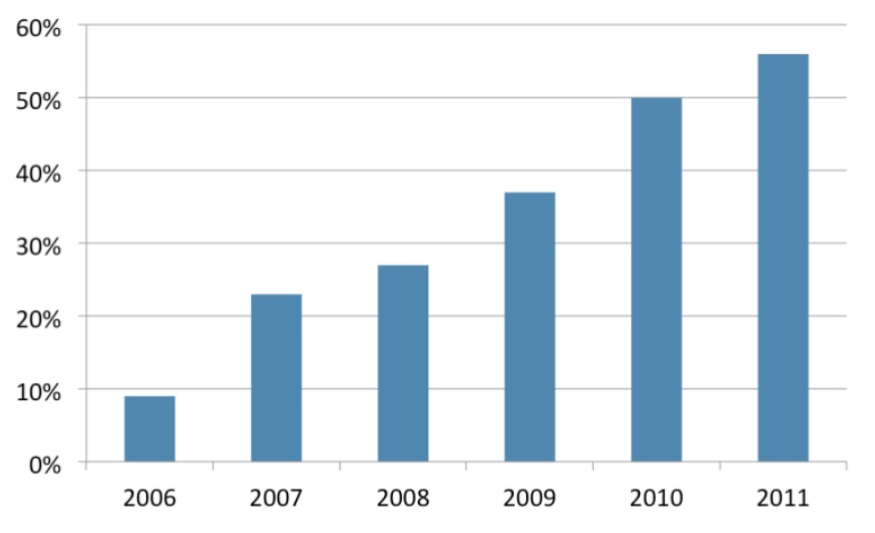
\includegraphics[width=0.9\textwidth]{images/json_support}
\captionof{figure}{Growth in percentage of APIs with JSON support}
\end{center}

Two out of number of possible data transport formats have been reviewed. According to projects requirements most suitable format decided is JSON. It less verbose, easy to be processed and will work faster on relatively slow mobile network.

\subsection{Comparison of available database systems}

There are several solutions on the market related to data storage, management and maintenance. Class of database management system will be in charge of data storage of the project.

\subsubsection{Oracle Database}

Oracle software package contain wide range of the functions for development on Java, access of the data over the Internet and simultaneous access optimization. One of the main disadvantages of this DBMS is a complexity of management and administration.

Among general properties of DBMS there are following

\begin{itemize}
	\item Hight reliability
	\item Ability to split large databases to partitions(large-database partition) 
	\item Existence universal mean of information security
	\item Effective methods of minimization of time for data querying 
	\item Indexes for binary representations
	\item Paralleling operations in querying
	\item Existence of wide spectrum of tools for development, monitoring and administration
	\item Web technologies friendly
\end{itemize}

Orientation on web technologies is one of the main directions of the Oracle's movement. Related to that could be mentioned following packages. interMedia for processing of data in multimedia formats and Jserver -- embedded tool for integration of Java language with relational databases.

\subsubsection{MySQL Server}

MySQL is a free DBMS. MySQL is a property of Oracle Corporation since Sun Microsystems, has been bought by it. MySQL released under GNU General Public License and under commercial license. Developers implement new features by request of users with commercial license, because of this mechanism even in early versions replication mechanism was realized.

MySQL is a good solution for small and medium applications. Usually MySQL is used as a server to which local and remote clients connect but also in distributive included solution for embedding databases into applications.

Flexibility of DBMS is enabled by support of relatively wide amount of storage engines: MyISAM that supports fulltext search as well as InnoDB that supports transactions on a level of separate records. Because of open architecture and GPL license new types of storage engines appear.

\subsubsection{Redis}

Redis is an open source key-value data store. Redis store it's data in memory and includes mechanism of snapshots and journaling system for persistent storage. Datastore supports messaging pattern publish-subscribe, which enables clients to create channels, push messages to them and  subscribe to channels.
Redis supports master-slave data replication and transactions. Data store belongs to so called NoSQL databases. In contradiction to previous DBMSes which are relational databases that supports SQL querying, NoSQL is a simple store that doesn't support complicated queries. Those properties makes Redis faster and more reliable.

NoSQL databases rely on BASE paradigm. That means storage is Basically Available Soft-state and Eventual consistent. Those kind of databases put Availability on the first place.

\subsubsection{MongoDB}

MongoDB is document driven schemaless database system. As Redis MongoDB is a NoSQL DBMS, which means it doesn't support SQL queries. But in contrast to Redis MongoDB is not a key-value store, it supports simple and complex querying based on comparison of querying statements to stored data.

MongoDB is released under open source license. DBMS supports replication for data protection in case of emergency. 
In addition MongoDB supports one special kind of index that don't support mentioned kinds of databases out of the box. That special index related to approximate querying of geolocation data and called 2D index. It allows to find records that contain position information in two-dimension space near given position with some approximation faster than just calculating difference with come other tools.

Relational SQL solutions such as MySQL and Oracle supports complicate relations between data entities. Querying of such data is performed by complex queries such as SQL.

Those kinds of databases are suitable for complex data relations storage.
Mostly Relational databases comply with ACID principle.

Relational databases usually require strong schemas of stored data to be able to make relations determinant and query relational data properly.
Usually provides solutions for scalability and recovery from errors as MySQL and Postgre

NoSQL databases relies on BASE paradigm. That means storage is Basically Available Soft-state and Eventual consistent. Those kind of databases puts Availability on the first place.

In general NoSQL databases is second generation of databases that take advantage of increased computation power and resources of new hardware systems.

Even relatively recently developed NoSQL systems proven it's work in many fields of enterprise usage.

Usually those databases have build-in solutions for redundant data storage for scalability and crash recovery. For instance MongoDB has full spectrum of replication solution that comes in default package.

MongoDB has additional support for so called 2D indexes that used for 2D queries. Geolocagion data of Points of interest could take advantage of those indexes for making queries based on approximate geo-position.

MongoDB is open source database licensed under GNU AGPL.

This project doesn't have complex data to be stored so it doesn't forced to use relational model. NoSQL solutions are usually more lightweight and scalable.

\subsubsection{Choice of the database system}

All of the mentioned database systems have tools technologies to fulfill requirements. Relational database systems is more suitable for complex data which is not in the requirements. Redis and MongoDB is a reliable solutions that could be chosen for project task. Due to addition means of querying data, support of 2d index that could be used for the system and free open source license MongoDB is chosen for current project.

\subsection{Comparison of available programming languages}

Backed application should use on of the technologies for API realization. Chosen technology must be able to implement mechanisms decided to be used for API, including REST principle and messaging formats.

There are number of stacks suitable for this purpose.

\subsubsection{Ruby}

Ruby on Rails(RoR) is a framework for programming language Ruby. RoR utilizes MVC principle for web applications. Framework enables developer to implement web based server applications, including REST services with less code.

Ruby on Rails provides tools for simplification of development of authorization and authentication, database handling and others.

\subsubsection{JavaScript}

NodeJS is a server-side technology that use JavaScript as language for it's applications. It's lightweight and event driven, but has number of drawbacks. Spread of server-side JavaScript is new and not widely used. Consequently there are some number of libraries and tools but that number are not that large and usually of not needed quality as soon as technology is not widely used for enterprise applications.

Express is a server JavaScript framework for quick development of JavaScript Web applications. Express provides toolkit for development of REST applications as additional functionality for Authorization and Authentications, encryption, etc.

NodeJS and Express stack doesn't have build in tools for deployment and monitoring applications.

NodeJS has package management tools for enabling extra functionality by use of third party libraries.
Code is executed by NodeJS server application.


\subsubsection{PHP}

PHP one of the most popular programming languages for the web (along with Java and languages of ASP.NET) because of it's simplicity, execution speed, rich functionality, cross-platforming and open source PHP license.

PHP was originally designed for development of web applications. It includes build-in tools for handling HTTP requests including parts of it such as cookies, HTTP headers, session handling, authentication, handling file upload, etc.

PHP has several comprehensive frameworks for complex web applications development such as CodeIgniter and Symphony. They include tools for object mapping, database connectivity, MVC paradigm implementation and others.

One of the biggest sites that use PHP are Facebook, Wikipedia, VK.

\subsubsection{Python}

Python is a high-level programming language of general purpose. Python phylosophy emphasizes code readability and minimization, syntax allows developers to use fewer lines of code for the simillar tasks compared Java or PHP. 

Python supports multiple programming paradigms, including object-oriented, imperative and functional programming. Python applications run using Python interpreters which are available for many operating systems. Python runs on server by use of Python interpretator and Web Server such as Apache.

Python first appeared in 1991 and wasn't designed to implement web applications. There are number of frameworks such as Django and Flask developed for Python, they enables developers to implement web-based applications and services easily and enables to use extra functionality for handling databases, authorization and authentication, encryption and so on easily.

Python has package management tool that provides convenient way of external libraries usage.
 

\subsubsection{Java}

Java is an object-oriented programming language developed by Sun Microsystems and acquired by Oracle Corporation. Applications written in Java usually translated to special byte-code which runs on Java Virtual Machine(JVM). That way of application execution makes programs almost in depended of hardware architecture it runs on.

Java is used by enterprise sector frequently. Consequently Java has vast collection of tools and libraries for handling huge majority of problems.

Compiled Java code could be executed on different Java Web Servers as well as standalone using JVM only.

Java developers could take advantage package managing and project build with dependence handling using different tools including Maven and Gradle.

Java applications could be scaled and monitored with support of different Java Web servers and Service 
Buses. One of the is Oracle Web Service Bus, which provides extra features for deployment, monitoring, scaling and other advantages.

Spring MVC is a contemporary framework for development Web applications using Java language. It supports operations for implementation REST services. Object mappers supports Java object translation to different formats for messaging between client and server.

Spring MVC could take advantage of existing Java libraries to enable different kinds of functionality such as Authorization, Authentication, encryption, monitoring and different databases support.


\subsubsection{ASP.NET}

ASP.NET is a server-side Web application framework designed for Web development to produce dynamic Web pages. It was developed by Microsoft to allow programmers to build dynamic web sites, web applications and web services.

\subsubsection{Choice of programming language}

All of the mentioned solutions are suitable for the project tasks. Named technologies relatively similar in terms of abilities they provide for developers. 
Java has been chosen as programming language for this project along with Spring MVC framework. Java and Spring framework are released under open source license have comprehensive documentations. Spring MVC have set of tools for faster development of the web services.

\subsection{Choice of mobile platform}


\subsubsection{Android OS and compatible devices}


Android operation system potentially supports whole spectrum of operations with hardware needed to get project implemented including but not limited to geolocation, networking, data processing. 

Android OS has developers SDK that provides possibility to develop third party application and supports number of different languages of application development e.g. Java, C and C++.

Even thought required options are possibly supported devices compatible with Android OS must not to have needed hardware components, which neglect goals of this project.

\subsubsection{iPhone and iOS}

iPhone 4S or newer has build in hardware modules for fast and precise geolocation recognition compared to other devices. iPhone has two chips for location recognition AGPS and GLONASS. Combined they make geolocation determination more accurate and fast.

iPhone has communication options of latest technologies, which enable it to utilize API over Internet, and use contemporary technologies for faster data transfer. 

Device has relatively strong computation power and resources that make it suitable for generation and processing required data.

iOS as an operation system of iPhone devices have developers SDK which enables developers to use whole spectrum of hardware parts needed for this project including geolocation, networking and data processing to develop third party application.

\subsubsection{Choice of mobile platform}

Due to strong computation power guaranteed persistence of required hardware options, existence of developers SDK makes it possible to develop third party applications using this hardware, iPhone is chosen as platform for Points of interest creation and as API client.


\chapter{Realisation of API}

\section{API design}

To provide interactions based on client-server model API should enable to manage two kinds of objects which are:

\begin{enumerate}

	\item Points of interest or places is main subject of communications. Stores geolocation data and additional info for the user.
	\item	User object to enable authentication and authorization for the clients.

\end{enumerate}

API must support full spectrum of CRUD operations of points of interest for authorized clients.
API must support operations of creation and reading of user objects to be able to distinguish data of different clients.

\subsection{General structure}
Service provide four operations on places for user 'create', 'read', 'delete', 'update'.

Operation 'create' adds place to user’s places:
	\begin{itemize}
		\item input: a place object
		\item output: text informing that place was added to user supplemented with created place object
	\end{itemize}

Operation 'read' returns places of the user
	\begin{itemize}
		\item input: place id or nothing
		\item output: places objects
	\end{itemize}

Operation 'delete' removes place from user’s places
	\begin{itemize}
		\item input: place id
		\item output: none
	\end{itemize}

Operation 'update' updates place for user
	\begin{itemize}
		\item input: place id
		\item output: none
	\end{itemize}

Service provides 'create' operation on users

Operation 'create' adds user to users collection
	\begin{itemize}
		\item input: none or user object
		\item output: text informing that user created supplemented with created user object
	\end{itemize}

Service provides 'read' operation of events places.

Operation 'read' returns places of the event
	\begin{itemize}
		\item input: event id
		\item output: places objects
	\end{itemize}


\subsection{Response codes}

HTTP supports response codes to acknowledge client about requested operation status. Some of them supported only by some operations, for instance code “201” means that entity is created and couldn't be used in response of “GET” request.

Current project requires CRUD operations support and following codes will be needed to provide client information about operation status. 
\begin{itemize}
	\item “200” is “OK” will be returned in case requested operation succeeded. That could be usual data retrieval or operations of updating or deleting of data.
	\item “201” is “Created” will be returned in case requested operation of object creation is succeeded. 
	\item “400” is “Bad request” will be returned in case of undocumented set of data in request
	\item “401” is “Unauthorized” will be returned when client tries to get data which is not belong to him.
	\item “404” is “Not found” will be returned when requested data doesn't exists.
\end{itemize}


\subsection{Resources}
Following resources for designed API were determined.

\begin{itemize}
	\item /places is a container of all 'places' for current user
	\item /places/{place-id} is a place with id 'place-id'
	\item /users - is a container for all 'users' in the system
	\item /events/{event-id}/places is a place with id 'place-id'
\end{itemize}

\subsection{Request and response structure}
\label{sec:reqstructure}

Data transfered between API and client is structured in the following way, depending on requested resource.

\begin{lstlisting}
- /places - list of all places
- /places/{place-id} - one place
	- title - name of the place
	- latitude - geographical latitude
	- longitude - geographical longitude
	- altitude - altitude 
	- horizontalAccuracy - horizontal accuracy 
				of position determination 
	- verticalAccuracy - vertical accuracy
				of position determination
	- date — date of creation 

- /events/{event-id}/places - list of event places

- /users - only for POST requests to create new user
	- id - unique id used for user’s Authorization
\end{lstlisting}

\subsection{Resource representations}
According to requirements analysis and possible messaging formats comparison representation of the resources defined in JSON.

\subsection{API usage}

\subsubsection{Users}

To create new 'user'

\begin{lstlisting}

POST to /users

Possible status codes

- 201 - Created (user added to users collection)

\end{lstlisting}

\subsubsection{Points of interest}

\begin{lstlisting}

To add 'place' to user’s places

POST to /places

Possible status codes

- 201 - Created (place added to users places)
- 400 - Bad request (wrong data)
- 401 - Unauthorized (wrong or absent user credentials)

To update 'place' with id place-id of user 

PUT to /places/{place-id} 

Possible status codes

- 200 - OK (place information updated)
- 400 - Bad request (wrong data)
- 404 - Not found
- 401 - Unauthorized (wrong or absent user credentials)

To delete 'place' with id place-id of user 

DELETE to /places/{place-id}

Possible status codes

- 200 - OK (place removed from user’s places)
- 400 - Bad request (wrong data, place not found)
- 404 - Not found
- 401 - Unauthorized (wrong or absent user credentials)

To retrieve 'places' of user 

GET to /places

Possible status codes

- 200 - OK 
- 400 - Bad request
- 401 - Unauthorized (wrong or absent user credentials)

To retrieve 'places' of the event with id event-id 

GET to /events/{event-id}/places

Possible status codes

- 200 - OK 
- 400 - Bad request (wrong data)
- 404 - Not found

To retrieve 'place' with id place-id of user 

GET to /places/{place-id}

Possible status codes

- 200 - OK 
- 400 - Bad request (wrong data)
- 404 - Not found
- 401 - Unauthorized (wrong or absent user credentials)
\end{lstlisting}

\subsection{API call example}

In response of get saved places request server returns data similar to the following

\begin{lstlisting}

[{
          "title": "Cycle parking",
          "latitude": 43.1256,
          "longitude": 12.5314,
          "altitude": 12,
          "icon": "cycle",
          "date": "2015-03-11 12:57"
        },
        {
          "title": "Hotel",
          "latitude": 42.1256,
          "longitude": 12.5214,
          "altitude": 15,
          "icon": "house",
          "date": "2015-03-10 10:07"
        }]

\end{lstlisting}

Response could be different depending on data stored for particular user. Structure of the response defined in respected section "Request and response structure" (\ref{sec:reqstructure})

To prevent attacks based on capturing of traffic between client and server encryption must be present by use of TLS certificate.
Authentication is enabled by HTTP authentication technology Basic HTTP Authentication.

\section{API realization}


\subsection{Model-View-Controller}
Server application will use MVC principle. 

\subsubsection{Models}

Application uses only two classes. First is Places for description Points of interest. This class is used as well as data model for database storage and represent message message structure of respected API request.

Second class belongs to Users for identifying Places with users and for Authentication.

Models are mostly represented by classes. Models for database will consists some extra parameters for handling databases queries and proper storage objects in data store. Such parameters mostly used for proper work of indexes and additional formats of the data store.

Application structure is represented on the following picture

\begin{center}
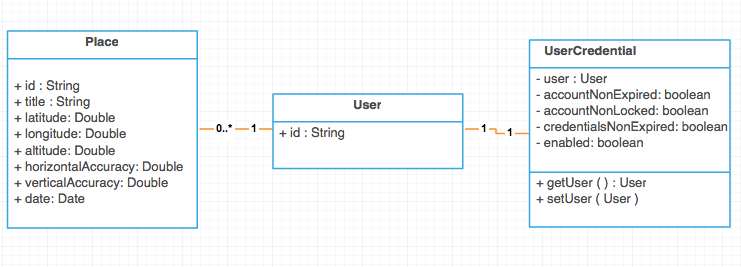
\includegraphics[width=1.0\textwidth]{images/uml/uml_server}
\captionof{figure}{Application structure}
\end{center}

UserCredential class is a class that implements build-in Spring MVC UserDetails interface. This interface is used for implementation classes that responsible for Spring authentication and authorization mechanisms. 

\subsubsection{Views}

Views are automatically generated by converting objects to JSON format by Spring MVC using Http Message Converters. 

\subsubsection{Controllers}

Controllers are responsible for routing requests to particular endpoints. Each function in respective Spring REST controller is responsible for one or several type of requests. Each controller is responsible for particular resource type.



\section{Build}

Widespread Java infrastructure requires addition solution for building project. Projects have to be build and deployed. There are number of solutions that perform this task. Several of the number of such solutions are  Maven and Gradle.
Those build systems are quite similar and suitable for general purposes and requirements of the project.

Maven is used for this project. Typical maven requirement is presence of pom.xml file which describes dependences of the project and could contain code like following.

\begin{lstlisting}
<?xml version="1.0" encoding="UTF-8"?>
<project xmlns="http://maven.apache.org/POM/4.0.0"
 xmlns:xsi="http://www.w3.org/2001/XMLSchema-instance"
    xsi:schemaLocation="http://maven.apache.org/POM/4.0.0
 http://maven.apache.org/xsd/maven-4.0.0.xsd">
    <modelVersion>4.0.0</modelVersion>

    <groupId>org.springframework</groupId>
    <artifactId>gs-spring-places-api</artifactId>
    <version>1.1.0</version>

    <parent>
        <groupId>org.springframework.boot</groupId>
        <artifactId>spring-boot-starter-parent</artifactId>
        <version>1.2.3.RELEASE</version>
    </parent>

    <properties>
        <java.version>1.8</java.version>
    </properties>

    <dependencies>
        <dependency>
            <groupId>org.springframework.boot</groupId>
            <artifactId>spring-boot-starter-web</artifactId>
        </dependency>
        <dependency>
            <groupId>org.springframework.boot</groupId>
            <artifactId>spring-boot-places-api</artifactId>
            <scope>test</scope>
        </dependency>
    </dependencies>


    <build>
        <plugins>
            <plugin>
                <groupId>org.springframework.boot</groupId>
                <artifactId>spring-boot-maven-plugin</artifactId>
            </plugin>
        </plugins>
    </build>

</project>
\end{lstlisting}

Dependences mentioned in respected section automatically downloaded and included in the project by Maven.



\section{Deployment and isolation}

Application is stated to be scalable and easy to be deployed. That requirement comply with principle of microservices architecture. Such an architecture takes care of libraries environment required software versioning and separate component isolation and independance of those requirements.

That principle from development to production mirrors how cargo was shipped prior to the invention of intermodal shipping containers. At the origin, cargo was manually loaded one piece at a time onto the truck or train that carried it to the port. At the port of origin the cargo was unloaded onto the dock.

Containerization dramatically changed the ship. All non-bulk cargo is now packed into standard shipping containers, which can be carried by truck, trains and ships. The contents of the container are never touched in transit. In other words, the shipping container encapsulates it’s contents. It has become the standardized API of cargo.

One of the solutions of the containerization principle in software is Docker. Docker is a new way to containerize applications that is becomingly increasingly popular. It allows you to package a microservice in a standardized portable format that’s independent of the technology used to implement the service. At runtime it provides a high degree of isolation between different services.

Docker runs natively on Linux with kernel 3.10 or higher which is used as production environment for this project.

To run deploy and run implemented API application following Docker configuration could be used.

\begin{lstlisting}
FROM dockerfile/java:oracle-java8
EXPOSE 8080
CMD java -jar app.jar
ADD target/app-api-1.0.1-SNAPSHOT.jar data/app.jar
\end{lstlisting}

During build required Java environment will be installed. Target compiled application file will be copied. When container is started target application will be run and required port will be exposed.

Another container needed to be run for proper work of API application is official MongoDB container which doesn't require tuning.

Alternatively software could be run without containerization using JVM and MongoDB daemon.


\section{Security and encryption}

For prevention Man-in-the-Middle attacks, security encryption between server and client could be used so data enabled by API is meaningless even captured by hacker.

To make use of TLS server could use certificate for messages exchange.  The client and server agree on various parameters used to establish the connection's security. Basic procedure for that establishing is following.

The handshake begins when a client connects to a TLS-enabled server requesting a secure connection and presents a list of supported cipher.

From this list, the server picks a cipher and hash function that it also supports and notifies the client of the decision.

The server usually then sends back its identification in the form of a digital certificate. The certificate usually contains the server name, the trusted certificate authority and the server's public encryption key.

The client may contact the server that issued the certificate and confirm the validity of the certificate before proceeding.

In order to generate the session keys used for the secure connection, the client encrypts a random number with the server's public key and sends the result to the server. Only the server should be able to decrypt it, with its private key.

From the random number, both parties generate a 'master secret' and then negotiate a session key for encryption and decryption.

Security encryption established by installation of the TLS certificate.



\chapter{Realization of mobile application}

\section{Application Wireframes}

Wireframing is a technology which dramatically increases speed of interface development on early stages. Moreover it downs coast of any changes made in the beginning of design.

That's why firstly wireframes of mobile application have been developed. They do not contain exact proportions of elements and screen but make it possible to overview elements position.

\clearpage

\begin{center}
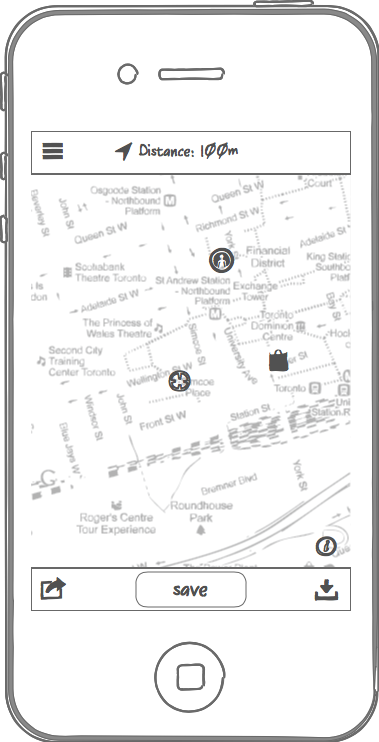
\includegraphics[width=0.5\textwidth]{images/wireframes/main_screen}
\captionof{figure}{Main application screen wireframe}

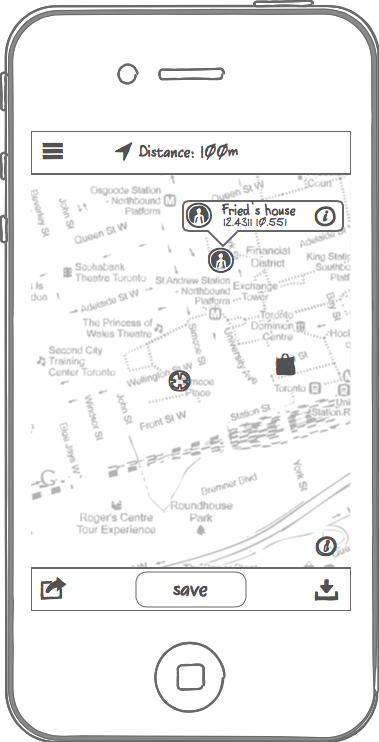
\includegraphics[width=0.5\textwidth]{images/wireframes/main_screen_detail}
\captionof{figure}{Main application screen with details wireframe}

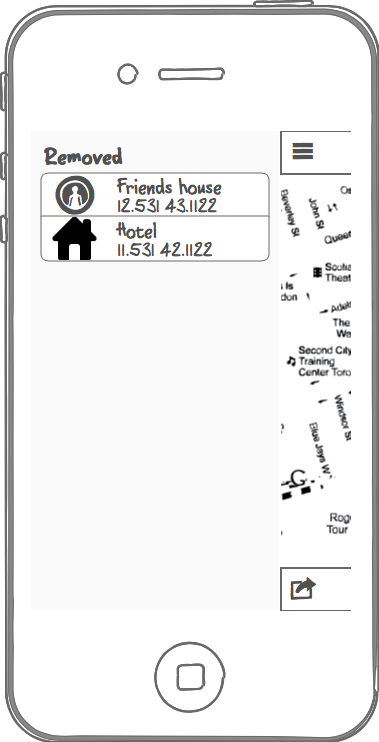
\includegraphics[width=0.5\textwidth]{images/wireframes/removed_places}
\captionof{figure}{List of removed places wireframe}

\end{center}

\section{Interface}

After detailed sketching of application interface it could be implemented in colors or in interface builder of development environment.

Following screenshots are actual images of the interfaces of the application.

\clearpage

\begin{center}
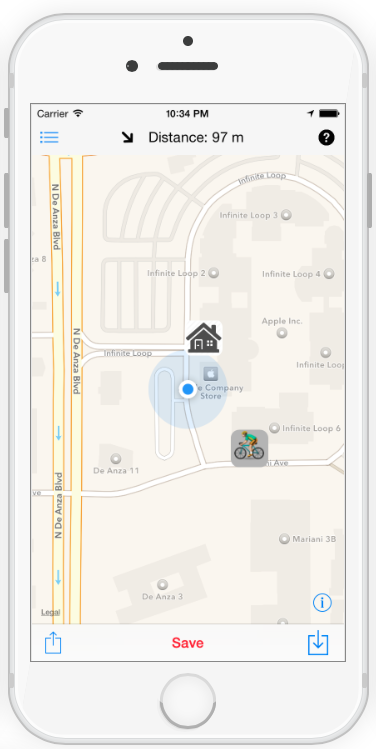
\includegraphics[width=0.5\textwidth]{images/screenshots/main_screen_device}
\captionof{figure}{Main application screen}

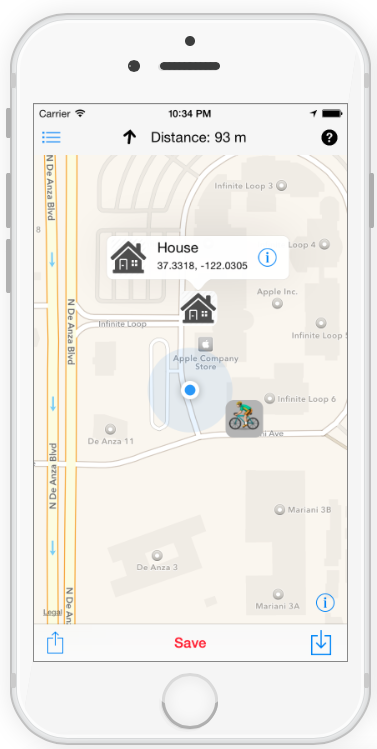
\includegraphics[width=0.5\textwidth]{images/screenshots/main_screen_detail_device}
\captionof{figure}{Main application screen with details}

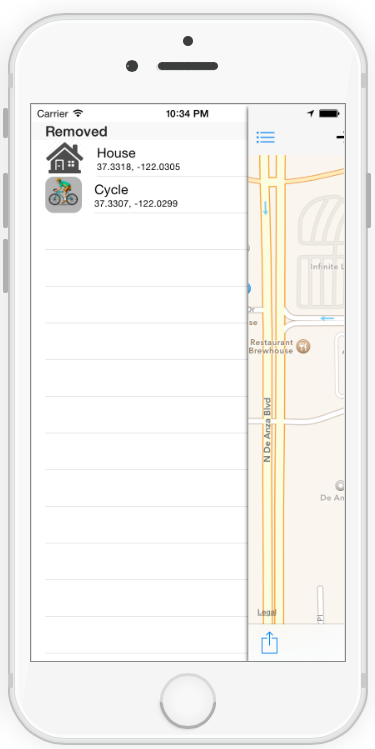
\includegraphics[width=0.5\textwidth]{images/screenshots/removed_places_device}
\captionof{figure}{List of removed places}

\end{center}


\section{Model-View-Controller}

Mobile application takes advantage of MVC principle. Model is represented mostly by classes. Classes are similar to server-side classes. Client-side application contain class Places, which represent user's data containing geolocation and meta information.

\begin{center}
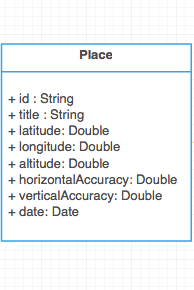
\includegraphics[width=0.5\textwidth]{images/uml/uml_places}
\captionof{figure}{Places class}
\end{center}

Most of the data that Place class stores make use of “location” object, which is instance of “Location” class representing geolocation in iOS developers SDK.


\begin{lstlisting}

class Place {
    
    var location: Location = Location()
    
    var latitude: CLLocationDegrees {
        return location.latitude
    }

    var longitude: CLLocationDegrees {
        return location.longitude
    }

    var coordinate: CLLocationCoordinate2D {
        return CLLocationCoordinate2D(latitude: latitude, longitude: longitude)
    }

    func setCoordinate(newCoordinate: CLLocationCoordinate2D) {
        self.location.latitude = newCoordinate.latitude;
        self.location.longitude = newCoordinate.longitude;
    }      

    var date: NSDate {
        return location.date
    }

}


\end{lstlisting}


\section{Networking}

Networking technologies
For network communication build-in libraries exist. For making development faster third-party libraries could be used for solving particular tasks. 

\section{Geolocation resolving}
iPhone has build in hardware and software for determination of device's location. Native libraries could be used for this task.

To resolve user location object of class CLLocationManager initialized. To respond to locations updates delegate of the created object complied with CLLocationManagerDelegate interface must be assigned. And actions required to be performed on location updates must be implemented in respective functions.



\chapter{Testing}

\section{Survey}

\subsection{Personas}

Representative group of potential users picked. Each separate personality called persona. Let's consider three of them.

\begin{itemize}
	\item Persona 1: male, 26 years, student of Masters program of CTU in Prague
	\item Persona 2: female, 23 years, student of CTU in Prague, hiking person
	\item Persona 3: male, 35 years, manager, traveler
\end{itemize}
All of the participants has iPhone what make them target group.

\subsection{Questionnaire}

\begin{enumerate}
	\item Would this application be useful for you?
	\item What would you add or remove from the application?
	\item Will you suggest application to somebody else?
\end{enumerate}


\subsection{Answers}

Persona 1

Q1: Yes

Q2: Searching and adding position by address

Q3: Probably

Persona 2

Q1: Yes, definitely

Q2: More precise position recognition

Q3: Yes

Persona 3

Q1: Probably

Q2: Coordinate system universalization

Q3: Yes, to friends

As seen most of the answers are positive related to use of software. It is expected as soon as personas were collected relatively different but interested in that piece of software to some extend, what rely on their lifestyle. Even though all of the participants are users of the iPhone there could be similar answers of users of different platforms, because use case is based on personality and shouldn't be affected by user device type.

\section{API Unit testing}

Unit testing is a process in application development, that allows developers to check validness of separate modules of source code of the application.

Ideology of unit testing is to develop tests for each non-trivial function of the application. That allows to check does or does not forthcoming changes of the source code would break functionality.

In case of possible future refactoring of the source code, unit tests ensures developer that application modules work as expected. Main principle of unit testing is calling methods and functions and check of the result for expected properties.

For instance response to the following request should contain error with code 404, meaning that requested place is not found.

\begin{lstlisting}
GET /places/10000 
\end{lstlisting}


Unit tests of the current project would cover most of the request of exposed API call. Spring MVC could use different libraries for test evaluation and by default uses JUnit.

\subsection{Unit tests development}

Example of unit test for user creation represented below.

\begin{lstlisting}
@Test
    public void createUser() throws Exception {
        String userJson = json(new User());
        
        this.mockMvc.perform(post("/users")
                .contentType(contentType)
                .content(userJson))
                .andExpect(status().isCreated());
    }
\end{lstlisting}

In the depicted example created post request to the resource /users. Response is checked for status containing information that object has been created, which represented in HTTP response codes by 201.


\section{Application test cases}


User test cases are developed in sake of  testing user behavior and assurance of proper work of the application. They are not applicable for API so developed for mobile application only.

\subsection{User test cases}

\textbf{Test case 1}

Test case name: Location determination

System: Mobile Application

Designed by: Ing. Timur Tatarshaov

Short description: Location determination

Pre-conditions:

The User looks at main screen of application

The User has accessed it by installing application on the mobile device

The mobile device has access to geolocation service

Step 1

Action: Launch of the Application

Expected system response: The application displays map and current Users location on it by representing blue circle with lighter outer circle.


\textbf{Test case 2}

Test case name: Location storage and remove

System: Mobile Application

Designed by: Ing. Timur Tatarshaov

Short description: Location storage and remove

Pre-conditions:

The User looks at main screen of application

The User has accessed it by installing application on the mobile device and launching application from mobile device launch screen. 

The mobile device has access to the Internet

The mobile device has access to geolocation service

Step 1

Action: Tap on "Save" button on application main screen

Expected system response: The application displays icon on the map representing stored user location.

Step 2

Action: Tap on just created icon

Expected system response: The application shows callout above stored place with additional information and "Actions" button

Step 3

Action: Tap on "Actions" button of the callout

Expected system response: The application shows actions sheet.

Step 4

Action: Tap on "Delete" button of the appeared actions sheet 

Expected system response: Previously created icon will be removed from the map.

Step 5

Action: Tap on "More" button on the left top corner of the application represented 

Expected system response: The Application shows left side-bar with list of removed earlier locations.



\chapter{Further development}

\section{API versioning and further development} 

Even though functions and technologies behind API implementation could change once designed, described and documented API functions shouldn't be changed to preserve compatibility with already implemented clients. New functions and methods could be added to implementation and documentation. 

There is possibility that API will be completely redesigned according to new philosophy or major changes. In this case API must preserve existing clients and assure their proper work. To solve this problem newly developed API URIs becomes prefixed with 'v' and version number. For instance next version of API could be hosted at URI started with.

\begin{lstlisting}
protocol://host:port/v1/
\end{lstlisting}

Such an approach widely used by big API providers such as Google, Facebook, Twitter, etc...

\section{API abuse usage prevention}


Even though communication between client and API is protected by encryption it's still vulnerable for abuse usage. API could be abused by undocumented access and filling up server recurses by spamming it with creation requests. That means hacker could access API in a not regular way and generate redundant traffic on API that normal client would never produce. 

Prevention from filling up server resources by abuse creation requests could be reached by installation of limits of such requests per user or per host.

Another type of abusing server application and API is denial of service(DoS) attack. It reached by frequent requests of the service and complete utilization either of server resources or communication channel capacity.

Those kinds of attacks could be prevented by installation system that catch suspicious traffic, filters it and install constrains and limitations for those kinds of clients.

That could be reached by installation and proper optimization Nginx web server, which could work as a proxy between web server and client.

\section{Extension to other platforms}

Even though one mobile platform has been used in project API is designed to be used by any number of various platforms and not tied to any particular. Among selected Android devices also often have required hardware for project implementation. Another class of mobile devices support Windows OS or Blackberry OS suitable for fulfilling requirements. 

There is one possibility to implement application for all of the mentioned devices at once. Such an approach utilizes devices ability to support web development technologies including JavaScript, HTML5 and CSS3. Applications developed using stated stack of technologies run in browser-like environment. One of the obvious advantage of such approach is cross-platform solution that developed only once and decreases costs of development for other platforms. Another advantage is compatibility with devices that has not been released yet will support mentioned stack and will need only browser-like environment to run application. 

PhoneGap is en open source framework that enables developers to implement cross platform mobile application using JavaScript, HTML5 and CSS3. PhoneGap compiles developed application to native application package for each supported mobile OS.

One of the drawbacks of such approach is slower application execution compared to natively developed application due to properties of used technologies. Another disadvantage of solution is that developed application could not take advantage of some hardware and software features provided by native development SDK.

Another way for implementation developed application on other platforms is usage of native SDK and languages of each platform. Such an approach will dramatically increase time of development. More over stack of technologies needed to be known by developers will be much wider. Each of the mentioned platform uses it's own language and framework for native application development.

Advantages of native development are in contradiction of the PhoneGap development. Implemented application will run faster and user interactions will be more satisfiable due to it's speed. Application could take advantage of different tools special for each OS and platform. Some of this tools are:
\begin{itemize}
	\item Live tiles of the application on the launch screen for Windows OS
	\item Widgets for Android OS, that allows to control application from the main screen
	\item Background run of the application for Android OS 
\end{itemize} 

Implemented API is generalized and simple to use. That enables developers of many of the products to implement API clients for other platforms. 

In such a case several client types would interact with the same API over the Internet.


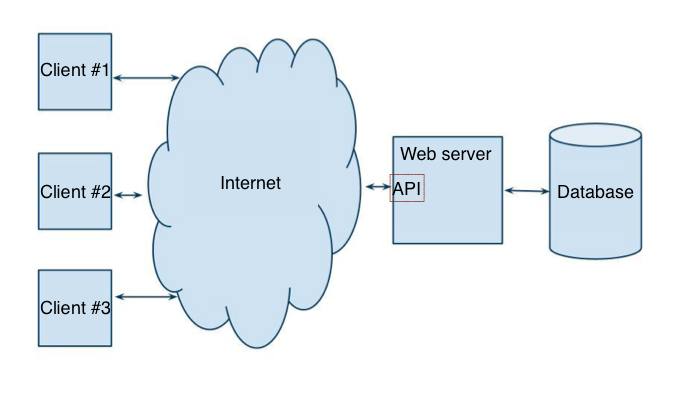
\includegraphics[width=0.9\textwidth]{images/extended_architecture}
\captionof{figure}{Multi client API interactions}



\setsecnumdepth{part}
\chapter{Conclusion}

In result of this project software solution was created. It aimed to remarkably ease process of the navigation of the unsettled places.
Software system has increased reliability, which is reached by synchronization of the data with remote server.

Advantages of the system are:
\begin{enumerate}
	\item	Cheap server side software required for system run
	\item	Scalable architecture of the server-side software
	\item	Designed and implemented API is suitable for different clients
	\item	Increased maintainability by usage of containerization 
\end{enumerate}

Disadvantages of the system are:

\begin{enumerate}
	\item	Low level of protection against server-side attacks
	\item	Low level of protection against API abuse
	\item	Low level of protection against third-party software usage
\end{enumerate}

Information system completely fulfills requirements of the thesis.
Use of the system is simple and intuitive. Implemented software solution can be useful for people who travel, used to have rest actively or have problems with orientation in space. 



\begin{thebibliography}{9}


\bibitem{auth}
  Tomas Vitvar, Authorization and Authentication lectures of MIE-W20. Available at: \url{http://humla.vitvar.com/slides/w20/lecture7.html}

\bibitem{geolocation}
  Ruizhi Chen and Robert Guinness,
  Geospatial Computing in Mobile Devices,
  Artech House,
  2014

\bibitem{restapidesign}
  George Reese,
  The REST API Design Handbook,
  Kindle,
  2012.

\bibitem{lamport13}
  Leonard Richardson,
  Mike Amundsen,
  RESTful Web APIs,
  O'Reilly Media,
  2013.

\bibitem{resttut13}
  THIJSSEN, Joshua and others. The RESTful CookBook [online]. 2012- 2014 [cit. 2014-10-23]. Available at: \url{http://restcookbook.com/}

\bibitem{restful}
  Leonard Richardson,Sam Ruby,
  RESTful Web Services,
  O'Reilly Media,
  2007

\bibitem{tls}
  Transport Layer Security protocol specification. Available at:  \url{https://tools.ietf.org/html/rfc5246}

\bibitem{ios}
  iOS \url{https://www.apple.com/ios}

\bibitem{swift}
  Swift \url{https://developer.apple.com/swift/}



\end{thebibliography}

%\bibliography{mybib}{}
%\bibliographystyle{csn690}
%\bibliography{mybibliographyfile}

\setsecnumdepth{all}
\appendix

\chapter{Terminology}
% \printglossaries
\begin{description}
	\item[User] User of mobile aplication holder and creator
	\item[Point of interest, Place] Data created by user and belonged to him, object of management using API
	\item[Client] Mobile device, property of user. Consumer of API. User interacts with API by means of the client
	\item[Server] Remote machine providing API entry point and API implementation. Includes set of technologies e.g. operation system, network stack, database to let API implementation work properly.
	\item[Database or data store] System for persistent storage of data on the server.
\end{description}

\chapter{Acronyms}
%\printglossaries
\begin{description}
	\item[XML] Extensible markup language
	\item[SOAP] Simple Object Access protocol
	\item[JSON] JavaScript Object Notation
	\item[CRUD] Create Read Update Delete
	\item[API] Application Programming Interface
	\item[HTTP] Hypertext Transfer Protocol
	\item[HTTPS] HyperText Transfer Protocol Secure
	\item[TLS] Transport Layer Security
	\item[SMTP] Simple Mail Transfer Protocol
	\item[PHP] Hypertext Preprocessor
	\item[SHA1] US Secure Hash Algorithm 1
	\item[GNU] GNU’s Not UNIX
	\item[GNU AGPL] GNU Affero General Public License
	\item[JVM] Java Virtual Machine
	\item[ACID] Atomicity, Consistency, Isolation, Durability
	\item[BASE] Basically Available Soft-state and Eventual consistent
	\item[JSON] JavaScript Object Notation
	\item[OS] Operation System
	\item[SDK] Software Development Kit
	\item[DBMS] Database Management System
	\item[WSDL] Web Services Description Language
	\item[TCP] Transmission Control Protocol
	\item[UDP] User Datagram Protocol
\end{description}


\chapter{Contents of enclosed CD}

%change appropriately

\begin{figure}
	\dirtree{%
		.1 readme.txt\DTcomment{the file with CD contents description}.
		.1 bins\DTcomment{the directory with executables}.
		.1 src\DTcomment{the directory of source codes}.
		.2 spring\DTcomment{the directory of API source codes}.
		.2 Spotty Finder\DTcomment{the directory of iOS application source codes}.
		.2 thesis\DTcomment{the directory of \LaTeX{} source codes of the thesis}.
		.1 text\DTcomment{the thesis text directory}.
		.2 thesis.pdf\DTcomment{the thesis text in PDF format}.
		.2 thesis.ps\DTcomment{the thesis text in PS format}.
	}
\end{figure}

\end{document}
